%
% 06_stueckweise_c1_kurven.tex -- Einfuhrung in den Satz von Jordan fuer stueckweise C^1-Kurven
%
% (c) 2026 Dominik Castelberg, Ostschweizer Fachhochschule
%
% !TEX root = ../../buch.tex
% !TEX encoding = UTF-8
%

\section{Der Fall stückweiser $C^1$-Kurven
\label{jordan:section:stueckweise_c1_kurven}}
\kopfrechts{Der Fall stückweiser $C^1$-Kurven}

Das Positive vorneweg: Der auf der Umlaufzahl basierende Beweis des Satzes von Jordan für reell-analytische Kurven bietet bereits eine fantastische Grundlage für den Beweis des Satzes von Jordan für stückweise $C^1$-Kurven.
Die Einführung von moderaten Singularitäten in Form von Ecken und Spitzen erfordert zwar einige zusätzliche Überlegungen, aber die Grundidee bleibt dieselbe: Die Umlaufzahl ist auf $\mathbb{C} \setminus \gamma$ lokal konstant und ganzzahlig, und die Mengen $I$ und $A$ können wie zuvor definiert werden.

\begin{definition}[Stückweise $C^1$-Kurve\label{jordan:definition:stueckweise_c1_kurve}]
    Eine stückweise $C^1$-Kurve mit endlich vielen Ecken und Spitzen ist eine stetige injektive Abbildung $\gamma: S^1 \to \mathbb{R}^2$ mit der Eigenschaft, dass eine endliche Zerlegung $0 = t_0 < t_1 < \ldots < t_n = 1$ von $S^1$ existiert, sodass $\gamma$ auf jedem offenen Teilintervall $(t_{k}, t_{k+1})$ regulär $C^1$ ist ($\gamma'(t)$ ist stetig und $\gamma'(t) \neq 0$).
    Zusätzlich existieren an jedem $t_k$ rechtsseitige und linksseitige Tangentenvektoren die unterschiedlich sein können. 

    \begin{itemize}
        \item Eine Ecke ist ein Punkt $t_k$, an dem die rechtsseitige und linksseitige Tangente nicht kollinear sind.
        \item Eine Spitze ist ein Punkt $t_k$, an dem die rechtsseitige und linksseitige Tangente kollinear, aber entgegengesetzt gerichtet sind.
    \end{itemize}
\end{definition}

\begin{figure}
    \centering
    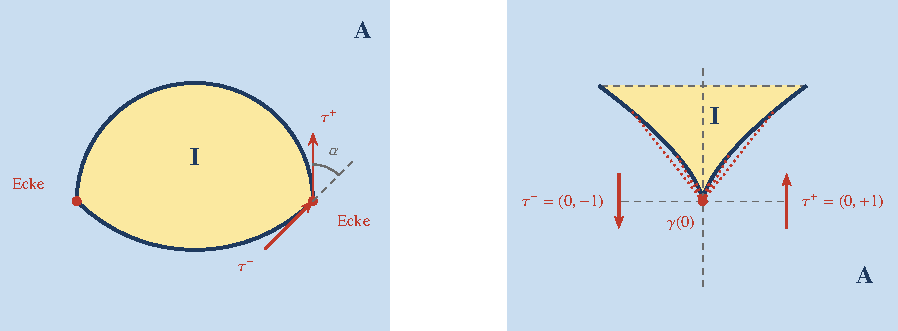
\includegraphics{papers/jordan/images/spitzen_ecken.pdf}
    \caption{Tangentenrichtung springt an Ecken (links) und kehrt an Spitzen (rechts).}
\end{figure}

Das grösste Problem bei stückweise $C^1$-Kurven ist die Tatsache, dass an Ecken und Spitzen keine eindeutige Tangente existiert, was die Eruierung der Tangentenwindungszahl, und damit auch die Berechnung der Umlaufzahl, erschwert.

Konkret verlieren wir folgende Bausteine:

\begin{itemize}
    \item \textbf{Hopfscher Umlaufsatz:} Er wurde für reguläre Kurven formuliert und ist auf die Existenz eindeutiger Tangenten bei jedem Punkt der Kurveangewiesen.
    \item \textbf{Tubulare Umgebung:} An einer Ecke ist der Normalenvektor nicht stetig, und somit ist die Abbildung der tubulären Umgebung nicht mehr wohldefiniert. 
        An einer Spitze kollabiert sie, weil die Normale ``umklappt''.
\end{itemize}

\subsection{Modifikationen des Umlaufzahl-Beweises}

Der Umlaufzahl-Beweis lässt sich mit geringem Aufwand auf stückweise $C^1$-Kurven übertragen, da das Integral über die Kurve $\gamma$ in Integrale über die glatten Teilbögen zerlegt werden kann:

\[
    \oint_{\gamma} f(\zeta) d\zeta = \sum_{k} \int_{\gamma | \left[ t_{k}, t_{k+1} \right]} f(\zeta) d\zeta
\]

wobei auf jedem glatten Teilbogen alles wohldefiniert ist. Punkte, die weder auf $\partial \gamma$ noch auf Ecken oder Spitzen liegen, sind die generischen Punkte. Ecken und Spitzen sind endlich viele spezielle Punkte auf $\gamma$

\begin{lemma}[Umlaufzahl für stückweise $C^1$-Kurven\label{jordan:lemma:umlaufzahl_stueckweise_c1_kurven}]
    Für jede stückweise $C^1$-Jordan-Kurve $\gamma$ mit endlich vielen Ecken und Spitzen und jeden Punkt $z \notin \gamma$ gilt: \begin{enumerate}
        \item Das Integral
        \[
            n(\gamma, z) = \frac{1}{2\pi i} \oint_{\gamma} \frac{d\zeta}{\zeta - z}
        \]
        ist wohldefiniert und ganzzahlig.
        \item $n(\gamma, \cdot)$ ist lokal konstant auf $\mathbb{C} \setminus \gamma$.
        \item $n(\gamma, z) = 0$ für hinreichend grosse $\left|z\right|$.
    \end{enumerate}
\end{lemma}

\subsection{Modifizierter hopfscher Umlaufsatz: Gauss-Bonnet für stückweise $C^1$-Ränder}

Der hopfsche Umlaufsatz muss angepasst werden, um Ecken und Spitzen zu berücksichtigen.
Sei $\gamma$ eine einfach geschlossene stückweise $C^1$-Kurve mit endlich vielen Ecken an $t_{1}, \ldots, t_{m}$ und endlich vielen Spitzen an $t_{m+1}, \ldots, t_{m+1}$.
An jeder Ecke $t_i$ definiert man den Aussenwinkel $\alpha_i$ als den orientierten Winkel zwischen der einlaufenden und auslaufenden Tangente (mit dem Vorzeichen: positive $\alpha_i$ für eine Linkskurve, negative $\alpha_i$ für eine Rechtskurve).
An einer Spitze ist der Aussenwinkel $\pm \pi$, die Kurve klappt also um.

\begin{satz}[Satz über die stückweise Totaldrehung (Gauss-Bonnet, polygonaler Randanteil)\label{jordan:satz:gauss-bonnet}]
\index{Satz!Gauss-Bonnet}%
    Für eine einfach geschlossene, positiv orientierte, stückweise $C^1$-Jordan-Kurve $\gamma$ gilt:
    \[
        \sum \int_{\text{glatte Teile}} \varkappa \ ds + \sum \alpha_i = 2\pi
    \]
    wobei die erste Summe über die glatten Teilbögen läuft und die zweite über die Aussenwinkel an Ecken und Spitzen.
\end{satz}


Dies ist der klassische Gauss-Bonnet-Satz für stückweise glatte Ränder in der Ebene. 
Der Beweis erfolgt durch Approximation der stückweise $C^1$-Kurve durch glatte Kurven, wobei an den Ecken kleine Bögen eingesetzt werden, und Grenzwertbildung. 
Die Krümmungsintegrale auf den eingesetzten Bögen konvergieren genau gegen die Aussenwinkel.

\subsection{Lokale Analyse an Ecken und Spitzen}

Um sicherzustellen, dass die Mengen $I$ und $A$ weiterhin komplett durch $\gamma$ getrennt werden, müssen wir garantieren können, dass die moderaten Singularitäten an Ecken und Spitzen keine ``Löcher'' in die Kurve reissen.

\subsubsection{Ecken}
Sei $p = \gamma(t_i)$ eine Ecke mit Tangentenvektoren $\tau^{-}$ und $\tau^{+}$.
In einer kleinen Kreisscheibe $B(p, \delta)$ zerlegt der Bogen $\gamma \cap B(p, \delta)$ die Kreisscheibe in zwei Sektoren: Einen mit Innenwinkel $\pi - \alpha_i$ und einen mit Aussenwinkel $\pi + \alpha_i$.
Die beiden Sektoren gehören zu den beiden Seiten von $\gamma$. Lokal gibt es also weiterhin eine wohldefinierte Innen- und Aussenseite, wenn auch nicht mehr durch eine einheitliche Normale beschrieben.

\subsubsection{Spitzen}
Sei $p$ eine Spitze mit Tangentenvektoren $\tau^{-}$ und $\tau^{+}$. Eine Puiseux-Entwicklung lokal um $p$ ergibt $\gamma(t) \approx p + \left( t^2 \tau, t^3 v + o(t^3) \right)$ für einen Vektor $v$ senkrecht zu $\tau$.
Die Kurve berührt sich in $p$ tangential und trennt die Umgebung in zwei Komponenten: Das ``Innere'' der Spitze, umschlossen von der Kurve, und das ``Äussere''. 
Der Umlaufzahl-Ansatz umgeht diese lokale Analyse weitgehend, weil das Integral
\[
    \oint \frac{d \zeta}{\zeta - z}
\]
für $z$ nahe $p$, aber nicht auf $\gamma$, über die ganze Kurve weiterhin sinnvoll bleibt.
Der Beitrag der Spitze selbst ist Mass 0, und stört entsprechend die Umlaufzahl nicht.

\subsection{Der Satz von Jordan für stückweise $C^1$-Kurven}

Mit diesen Modifikationen des Umlaufzahl-Beweises und des hopfschen Umlaufsatzes gewinnen wir unsere verlorenen Bausteine zurück, und der Beweis des Satzes von Jordan für stückweise $C^1$-Kurven kann analog zum Beweis für reell-analytische Kurven durchgeführt werden.

Die tubuläre Umgebung mag global nicht mehr existieren, aber lokal auf jedem glatten Teilbogen kann sie konstruiert werden. Der Wegzusammenhang von $I$ und $A$ folgt durch Konstruktion lokaler Tuben, die an Ecken und Spitzen überlappend zusammengefügt werden.

Die Totaldrehung der Tangente ist jetzt die Summe aus Krümmungsintegral und Aussenwinkeln. Die entscheidende Aussage, dass für eine einfache geschlossene Kurve mit positiver Orientierung die Totaldrehung $2 \pi$ beträgt, bleibt erhalten.